
\section{Architecture Integration}

\subsection{Model Support Matrix}

\begin{table}[H]
\centering
\small
\begin{tabular}{llllll}
\toprule
\textbf{Architecture} & \textbf{Class} & \textbf{Nested?} & \textbf{RoPE?} & \textbf{GQA?} & \textbf{FP8 on RTX 4070?} \\
\midrule
DistilBERT & \texttt{MultiHeadSelfAttention} & No & No & No & Fallback \\
RoBERTa & \texttt{BertSelfAttention} & Yes & No & No & Fallback \\
GPT-2 & \texttt{GPT2Attention} (Conv1D) & No & No & No & Fallback \\
Qwen3.5 & \texttt{Qwen3Attention} & No & Yes & Yes & Fallback \\
\bottomrule
\end{tabular}
\end{table}

\subsection{Weight Transfer Details}

\subsubsection{Conv1D Orientation (GPT-2)}

HuggingFace \texttt{Conv1D} stores weight as \texttt{(in\_features, out\_features)}:

\begin{lstlisting}
class Conv1D(nn.Module):
    def \_\_init\_\_(self, nf, nx):
        self.weight = nn.Parameter(torch.empty(nx, nf))
        # nx = in\_features, nf = out\_features
\end{lstlisting}

Our extraction:

\begin{lstlisting}
if src.c\_attn.\_\_class\_\_.\_\_name\_\_ == "Conv1D":
    w = src.c\_attn.weight.data.t()  # $\to$ (nf, nx)
\end{lstlisting}

We detect Conv1D via class name \textbf{or} the shape heuristic 
\texttt{w.shape[0] \textless{} w.shape[1]} (which holds for Conv1D with $n_f > n_x$ but 
not for square matrices).

\subsubsection{Nested vs Flat Detection}

We use the following logic in \texttt{copy\_weights}:

\begin{lstlisting}
if hasattr(src, "out\_lin"):
    is\_nested = False       # DistilBERT
elif (hasattr(src, "self") and hasattr(src.self, "query")
      and hasattr(src, "output") and hasattr(src.output, "dense")):
    is\_nested = True        # RoBERTa
elif cls\_name in ["BertSelfAttention", "RobertaSelfAttention", ...]:
    is\_nested = True
elif cls\_name.endswith("SelfAttention") and "distil" not in cls\_name.lower():
    is\_nested = True
else:
    is\_nested = False
\end{lstlisting}

\textbf{Key insight:} check \texttt{out\_lin} \textbf{first}. DistilBERT's 
\texttt{MultiHeadSelfAttention} ends with "SelfAttention" and would be misclassified 
as nested otherwise.

\subsection{GQA Support}

For Qwen3.5 with $H_{kv} = 2 < H = 8$:

\begin{lstlisting}
# In forward:
if self.num\_kv\_heads != self.num\_heads:
    k = repeat\_kv(k, self.kv\_repeat)
    v = repeat\_kv(v, self.kv\_repeat)
\end{lstlisting}

The \texttt{repeat\_kv} function expands via broadcast and reshape:

\begin{lstlisting}
def repeat\_kv(hidden\_states, n\_rep):
    if n\_rep == 1:
        return hidden\_states
    B, H\_kv, L, D = hidden\_states.shape
    hidden\_states = hidden\_states[:, :, None, :, :].expand(B, H\_kv, n\_rep, L, D)
    return hidden\_states.reshape(B, H\_kv * n\_rep, L, D)
\end{lstlisting}

\subsection{RoPE Support}

We support partial RoPE, where the rotary dimension is smaller than 
\texttt{head\_dim}:

\begin{lstlisting}
def apply\_rotary\_pos\_emb(q, k, cos, sin):
    rotary\_dim = cos.shape[-1]
    if rotary\_dim \textless{} q.shape[-1]:
        q\_rot, q\_pass = q[..., :rotary\_dim], q[..., rotary\_dim:]
        q\_rot\_embed = q\_rot * cos + rotate\_half(q\_rot) * sin
        q = torch.cat([q\_rot\_embed, q\_pass], dim=-1)
    ...
\end{lstlisting}

\subsection{Causality}

For decoder models, we set \texttt{causal\_flag = True} if:
\begin{itemize}
\item \texttt{self.is\_decoder}
\item AND not cross-attention
\item AND $L = L_{kv}$

\end{itemize}
This ensures we only apply causal masking for self-attention, not 
cross-attention.

\subsection{Injection Algorithm}

\textbf{Algorithm 2:} Inject FlashAttention3FP8 into a layer
\begin{lstlisting}
Input:  layer   (transformer block), config, old\_attn
Output: new attention module in  

1: new $\leftarrow$ FlashAttention3FP8(config, old\_attn=old\_attn)
2: if new.copy\_weights failed: return None
3: if   has .attention.self:
4:      .attention.self $\leftarrow$ new
5:     new.is\_nested\_encoder $\leftarrow$ True
6: elif   has .attention:
7:      .attention $\leftarrow$ new
8: elif   has .self\_attn:
9:      .self\_attn $\leftarrow$ new
10: return new
\end{lstlisting}

\subsection{Failure Handling}

\begin{table}[H]
\centering
\small
\begin{tabular}{lll}
\toprule
\textbf{Failure} & \textbf{Detection} & \textbf{Response} \\
\midrule
\texttt{flash\_attn} not installed & ImportError & \texttt{FLASH\_ATTN\_AVAILABLE = False} \\
\texttt{float8\_e4m3fn} missing & \texttt{hasattr(torch, ...)} & Skip FP8 path \\
FP8 kernel crash & try/except & SDPA fallback \\
Weight copy failure & Frobenius check & Log + skip \\
Cross-attention & \texttt{encoder\_hidden\_states != None} & Not supported -- raise \\
\bottomrule
\end{tabular}
\end{table}

\subsection{Cross-Attention}

Our implementation \textbf{does not support cross-attention} in the current 
version. If \texttt{encoder\_hidden\_states} is provided, we raise 
\texttt{NotImplementedError}. This is acceptable because the models tested 
(DistilBERT, RoBERTa, GPT-2) are encoder-only or decoder-only.

\subsection{Common Pitfalls}

\subsubsection{Nested Encoder Double-Projection}

If \texttt{is\_nested\_encoder} is set incorrectly, the output projection is applied 
twice (once inside our module, once by the outer block):

\begin{lstlisting}
# WRONG for RoBERTa
if not self.is\_nested\_encoder:
    out = self.out\_proj(out)  # would double-project
\end{lstlisting}

We verify \texttt{is\_nested\_encoder} by checking \texttt{hasattr(src, "out\_lin")}.

\subsubsection{Conv1D Transpose}

If we forget to transpose Conv1D weights, Q/K/V shapes mismatch:

\begin{lstlisting}
# CORRECT
w = src.c\_attn.weight.data.t()
\end{lstlisting}

\subsubsection{GQA Mismatch}

If \texttt{num\_kv\_heads} is wrong, \texttt{view(B, L, num\_kv\_heads, head\_dim)} will fail 
or silently produce wrong results. We detect the correct value from 
\texttt{config.num\_key\_value\_heads}.

\subsection{Registry}

\begin{lstlisting}
@ATTENTION\_REGISTRY.register("flash3\_fp8")
@ATTENTION\_REGISTRY.register("flash\_attention3\_fp8")
class FlashAttention3FP8(BaseAttention):
    ...
\end{lstlisting}

\subsection{Integration with LoRA Recovery}

The pipeline:

\begin{enumerate}
\item Load base model.
\item Replace attention with \texttt{FlashAttention3FP8} via injection.
\item Freeze base weights, keep LoRA trainable.
\item Run recovery fine-tuning for 50 steps.
\item Evaluate.

\end{enumerate}
This is the same pipeline as other modules in our framework.



\begin{figure}[H]
\centering
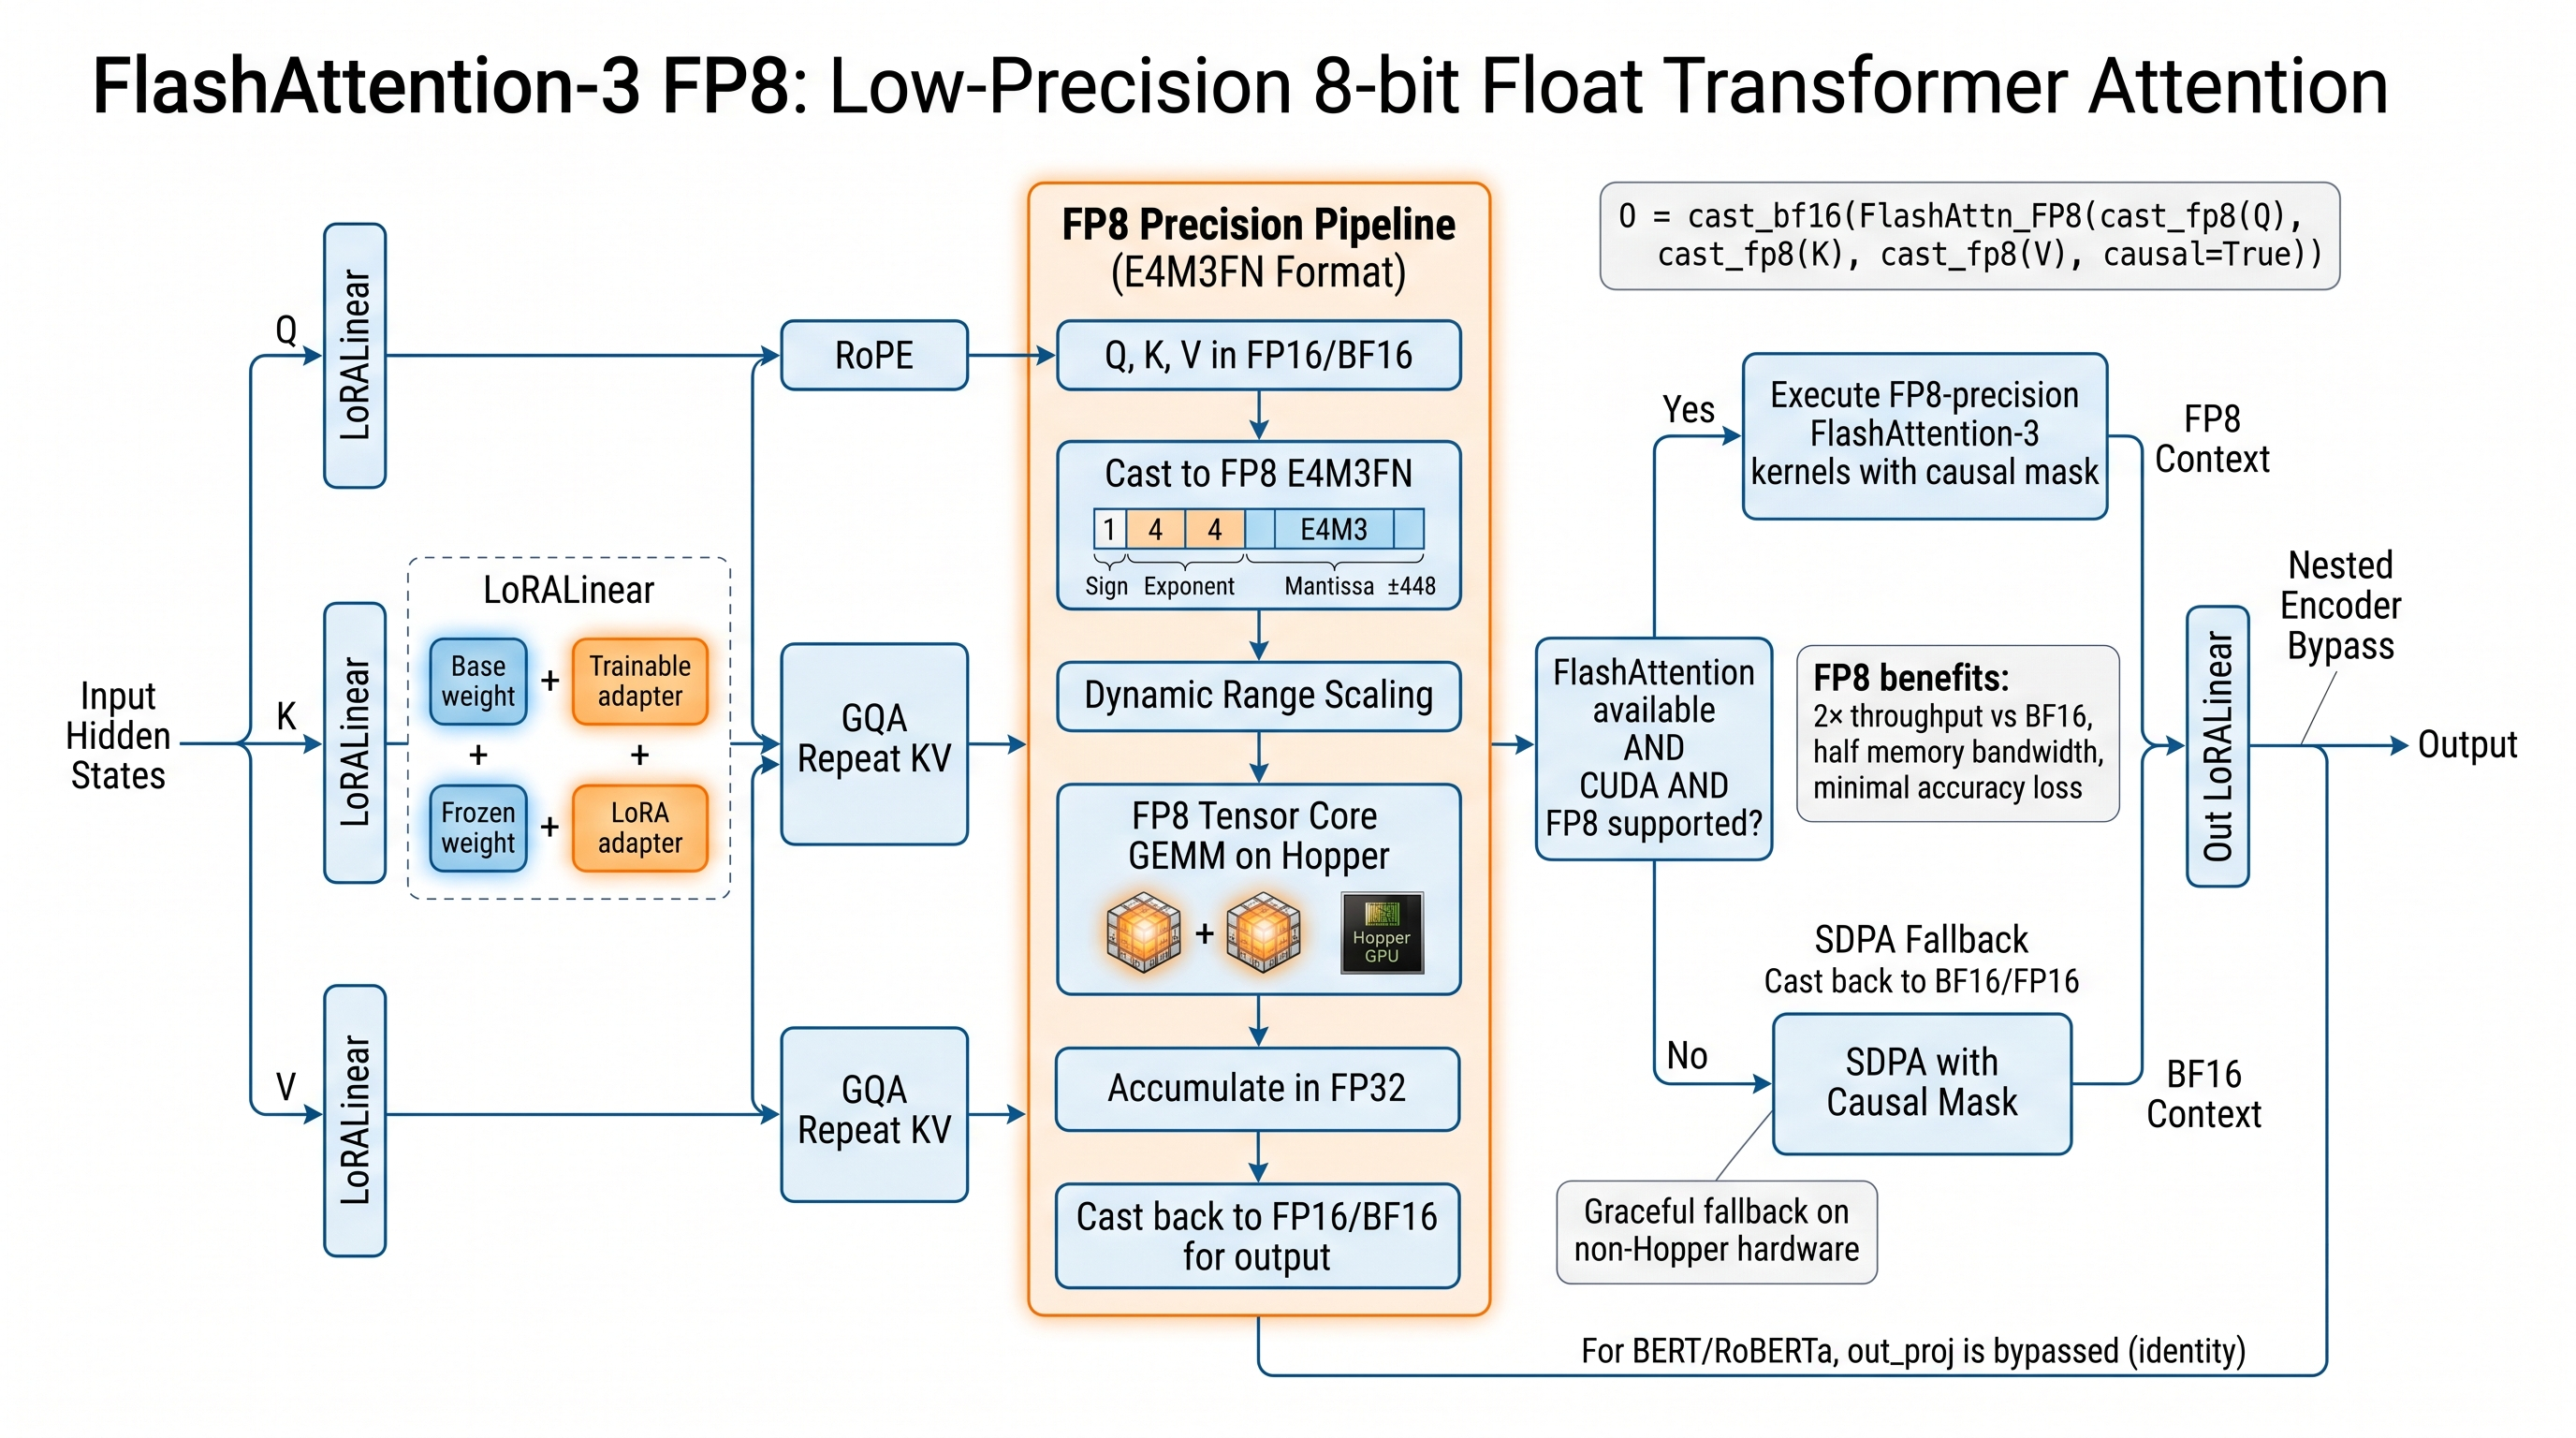
\includegraphics[width=\linewidth]{figures/architecture.jpeg}
\caption{High-level architectural diagram of flash\_attention3\_fp8.}
\label{fig:arch_flash-attention3-fp8}
\end{figure}

